\setchapterpreamble[u]{\margintoc}
\chapter{Proof-by-Action in Practice}
\labch{advanced}

In the previous chapters, we explained the core principles of our so-called
Proof-by-Action paradigm and especially its drag-and-drop actions, first through
basic and abstract examples in \refch{pba}, and then from a proof-theoretical
perspective in \refch{sfl}. The goal of this chapter is to provide a better
sense of what proofs by action/DnD look like in practice, and how they compare
to more traditional approaches to interactive theorem proving. To that effect,
we perform a case study of a few select examples, unrolling and commenting in
details one or many of their proofs. Although still basic, they are fully
fledged, concrete logical riddles or mathematical problems that one might give
as exercise to an undergraduate student learning formal proofs. Note that our
analysis will stay quite informal and opinionated: a more systematic approach
such as a user study would allow for a better evaluation of our paradigm, but at
the time of writing of this thesis the Actema prototype is not mature enough to
conduct a project of this scale.

The chapter is organized as follows: \refsec{edukera} studies a proof of a small
logical riddle in Actema, highlighting some benefits of our approach compared to
textual systems. \refsec{funcs} explores how basic properties about functions
between sets can be proved graphically, introducing the use of definitions in
addition to logical reasoning steps. In \refsec{arith} we prove equations in
Peano arithmetic, showing how one can incorporate additional actions into the
paradigm to deal with more specialized forms of reasoning: \emph{induction} and
\emph{automatic computation}.

\todo{ Explain that for all examples, we provide a Coq proof script that tries
  to follow the structure of the graphical proof, for the sake of comparison
  with a more standard text-based interface. But this would obviously compare
  differently with other textual approaches, e.g. Isar which is more
  declarative, and thus farther from the Proof-by-Action paradigm. }

\todo{ Maybe advise the reader to reproduce the examples herself? Supposes an
  easy way to setup and use coq-actema: nix seems like a good option, but maybe
  JsCoq could be doable with some efforts, and would provide an even more
  out-of-the-box experience.}

\section{Forward reasoning}\labsec{edukera}

% It is too early to perform a detailed case study comparing our approach
% to interactive theorem proving with others --- tactic-based,
% declarative, {\em etc}\dots~This is due primarily to the fact that
% our prototype is not mature enough; it cannot handle lemmas and
% implements a limited formalism. However some examples allow to get a
% glimpse of specificities and possible advantages of proofs by actions.

Our first example is a small logical riddle, which we borrow from a textual
educational system, Edukera~\sidecite{edukera}. One considers a population of
people, with at least one individual $h$, together with a single function
$\mother$ and one predicate $\rich$. The aim is to show that the two following
assumptions are incompatible:
\begin{itemize}
\item[(1)] $\forall x. \neg\rich(x)\lor \neg\rich(\mother(\mother(x)))$,
\item[(2)] $\forall x. \neg\rich(x) \limp \rich(\mother(x)).$
\end{itemize}
The original goal thus corresponds to the illustration of \reffig{edukera}.

\begin{figure*}
  \fbox{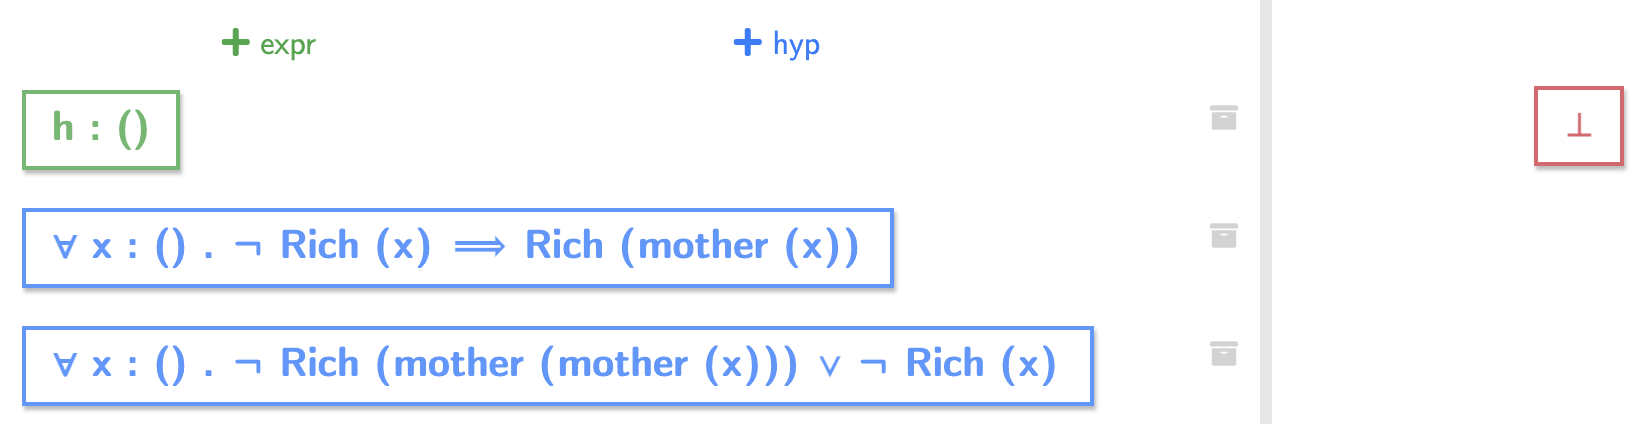
\includegraphics[width=1.3\textwidth]{edukera.png}}
  \caption{The beginning of an example due to Edukera}
  \labfig{edukera}
\end{figure*}

It is quite natural to approach this problem in a forward manner, by starting
from the hypotheses to establish new facts. And a first point illustrated by
this example is that DnD actions allow to do this in a smooth and precise
manner. A possible first step is to bring $h$ to the first hypothesis, to obtain
a new fact:

\medskip
$(3) ~\neg\rich(h)\lor \neg\rich(\mother(\mother(h))).$
\medskip

\noindent Double clicking on this new fact yields two cases:
\begin{itemize}
 \item[(4)~] $ \neg\rich(h)$,
 \item[(4')] $ \neg\rich(\mother(\mother(h)))$.
 \end{itemize}
Let us detail how one solves the
second one.

By bringing 
$\neg\rich(\mother(\mother(h)))$ on the premise of $\forall
x. \select{\neg\rich(x)} \limp \rich(\mother(x))$
one obtains

\medskip
$(6) ~\rich(\mother(\mother(\mother(h)))).$
\medskip

The next step is a good example where DnD actions are useful. By bringing this
new fact to the right-hand part of

\medskip
$(1)~\forall x. \neg\rich(x)\lor \neg\select{\rich(\mother(\mother(x)))}$
\medskip

\noindent
one immediately obtains a new fact

\medskip
$(7) ~\neg{\rich(\mother(h))}$.
\medskip

\noindent In other proof systems, this last step requires a somewhat intricate
tactic line and/or writing down at least the statement of the new fact.

One can then finish the case by combining $(7)$ and $(2)$ which yields
$$\rich(\mother(\mother(h)))$$ contradicting $(4')$. These two last steps each
correspond to a simple DnD. The other case, $\neg\rich(h)$, is quite similar.

% Such a simple example is not sufficient to provide significant metrics.
Note that once a user has understood the proof, the riddle is routinely solved
in less than a minute in Actema, which seems out of reach for about any user in
a tactic based prover. At least as important is the fact that the proof can be
performed without typing any text, especially no intermediate statement. 

To conclude this example, we propose in \reffig{edukera-coq} a complete proof of
the riddle formalized in the Coq proof assistant, which follows very closely the
structure of the graphical proof just outlined. To make the correspondence more
visible and ease the comparison, we interspersed the proof script with comments
of the form \texttt{(** [actions] *)}, where \texttt{[actions]} is a
sentence describing a sequence of actions in Actema that produces the same goal
transformation as the tactics preceding the comment. There are a few interesting
things to note:
\begin{itemize}
  \item We chose to name manually all the hypotheses introduced in the course of
  the proof. This is generally considered good practice in the Coq community,
  because it makes proof scripts easier to maintain. In our case it also has the
  advantage of expliciting which hypotheses are used exactly in the reasoning,
  something that an Actema user does with her pointing device when designating
  the blue items involved in an action. It appears clearly in
  \reffig{edukera-coq} that in a moderately long proof like this based mostly on
  forward reasoning, one needs to keep track of \emph{a lot} of names, which can
  be overwhelming for many users. This is especially true for beginners
  discovering Coq, because the syntax for assigning names, based on patterns
  like \texttt{[H | H]} that reproduce the subgoal structure, can induce a steep
  learning curve. Of course this problem is mitigated trivially in Actema, since
  names are not needed.

  \item There is no exact correspondence between the tactics of Coq and the
  actions of Actema: some tactics are simulated by multiple actions, and often a
  complex sequence of tactics can be simulated by a single action\sidenote{This
  was already noticed in \cite{PbP}, where clicking on a subformula can simulate
  a sequence of introduction rules of arbitrary length.}.
  
  For instance, line 23 does at the same time a specialization of the hypothesis
  $H_2 : \forall x. \neg \rich(\mother(\mother(x))) \lor \neg \rich(x)$ to the
  individual $h$ with the application \texttt{(H2 h)}, and a case analysis with
  the \texttt{destruct} tactic. In Actema this is performed in two steps, first
  by drag-and-dropping $h$ on $H_2$, and then by clicking on the resulting
  hypothesis\sidenote{This could also be achieved in two steps in Coq, by using
  the \texttt{specialize} tactic instead of the inlined application.}.

  In the other direction, a pattern of reasoning that occurs multiple times in
  the proof is the combination of $H_2$ with another hypothesis which
  contradicts one of the two cases, in order to deduce the truth of the other
  case. While it is captured straightforwardly in Actema with a single DnD
  between the contradictory statements, it requires in Coq a decomposition into
  many administrative steps:
  \begin{enumerate}
    \item first a case analysis with \texttt{destruct}, where the expression
    instantiating $H_2$ (e.g. $\mother(mother(h))$) needs to be written down
    explicitly, instead of being inferred automatically from unification;
    \item optionally focusing on the subgoal corresponding to the contradictory
    case if it is the right disjunct (line 56), which requires to know a
    somewhat idiosyncratic and infrequently used syntax of the tactic language;
    \item and finally expliciting the contradiction with \texttt{apply} and
    \texttt{exact}.
  \end{enumerate}

  \item More generally, the actions of Actema are more \emph{versatile} and
  \emph{context-dependent} than the tactics of Coq. For instance, click actions
  have a different effect depending on the main connective of the formula being
  clicked, but provide a unique interface for applying rules of natural
  deduction/sequent calculus. On the contrary, there is almost one tactic for
  dealing with each logical connective in Coq, e.g. \texttt{intros} for $\limp$
  and $\forall$, \texttt{split} for $\land$, \texttt{left} and \texttt{right}
  for $\lor$, \texttt{exists} for $\exists$, etc. The same remark applies to DnD
  actions, whose functionalities are provided in Coq by many different tactics:
  \texttt{apply \_}, \texttt{apply \_ in \_}, \texttt{pose proof},
  \texttt{specialize}, etc.
\end{itemize}

\begin{figure}[p]
  % \fontsize{8}{8.5}\selectfont
  % \begin{alectryon}
  % Generator: Alectryon
  \sep
  \begin{txt}
    \PY{c}{(*~Declaration~of~constants~used~in~the~statement~of~the~riddle~*)}\nl
    \nl
  \end{txt}
  \sep
  \begin{sentence}
    \begin{input}
      \PY{k+kn}{Context}~\PY{o}{(}\PY{n+nv}{i}~\PY{o}{:}~\PY{k+kt}{Type}\PY{o}{).}\nl
    \end{input}
  \end{sentence}
  \sep
  \begin{txt}
    \nl
  \end{txt}
  \sep
  \begin{sentence}
    \begin{input}
      \PY{k+kn}{Context}~\PY{o}{(}\PY{n+nv}{Rich}~\PY{o}{:}~\PY{n}{i}~\PY{o}{\PYZhy{}\PYZgt{}}~\PY{k+kt}{Prop}\PY{o}{).}\nl
    \end{input}
  \end{sentence}
  \sep
  \begin{sentence}
    \begin{input}
      \PY{k+kn}{Context}~\PY{o}{(}\PY{n+nv}{mother}~\PY{o}{:}~\PY{n}{i}~\PY{o}{\PYZhy{}\PYZgt{}}~\PY{n}{i}\PY{o}{).}\nl
    \end{input}
  \end{sentence}
  \sep
  \begin{sentence}
    \begin{input}
      \PY{k+kn}{Context}~\PY{o}{(}\PY{n+nv}{h}~\PY{o}{:}~\PY{n}{i}\PY{o}{).}\nl
    \end{input}
  \end{sentence}
  \sep
  \begin{txt}
    \nl
    \PY{c}{(*~Statement~of~the~riddle~*)}\nl
    \nl
  \end{txt}
  \sep
  \begin{sentence}
    \begin{input}
      \PY{k+kn}{Theorem}~\PY{n+nf}{rich\PYZus{}mothers}~\PY{o}{:}\nl
      ~~\PY{o}{(}\PY{k+kr}{forall}~\PY{n+nv}{x}\PY{o}{,}~\PY{o}{\PYZti{}}\PY{n}{Rich}\PY{o}{(}\PY{n}{x}\PY{o}{)}~\PY{o}{\PYZhy{}\PYZgt{}}~\PY{n}{Rich}\PY{o}{(}\PY{n}{mother}\PY{o}{(}\PY{n}{x}\PY{o}{)))}~\PY{o}{\PYZhy{}\PYZgt{}}\nl
      ~~\PY{o}{(}\PY{k+kr}{forall}~\PY{n+nv}{x}\PY{o}{,}~~\PY{o}{\PYZti{}}\PY{n}{Rich}\PY{o}{(}\PY{n}{mother}\PY{o}{(}\PY{n}{mother}\PY{o}{(}\PY{n}{x}\PY{o}{)))}~\PY{o}{\PYZbs{}/}~\PY{o}{\PYZti{}}\PY{n}{Rich}\PY{o}{(}\PY{n}{x}\PY{o}{))}~\PY{o}{\PYZhy{}\PYZgt{}}\nl
      ~~\PY{k+kt}{False}\PY{o}{.}\nl
    \end{input}
  \end{sentence}
  \sep
  \begin{txt}
    \nl
    \PY{c}{(*~Proof~of~the~riddle~*)}
  \end{txt}
\end{alectryon}

\begin{alectryon}
  % Generator: Alectryon
  \sep
  \begin{sentence}
    \begin{input}
      \PY{k+kn}{Proof}\PY{o}{.}\nl
    \end{input}
  \end{sentence}
  \sep
  \begin{sentence}
    \begin{input}
      ~~\PY{n+nb}{intros}~\PY{n}{H1}~\PY{n}{H2}\PY{o}{.}\nl
    \end{input}
  \end{sentence}
  \sep
  \begin{txt}
    \nl
    ~~\PY{l+s+sd}{(**~2~clicks~on~the~conclusion~*)}\nl
    \nl
  \end{txt}
  \sep
  \begin{sentence}
    \begin{input}
      ~~\PY{n+nb}{destruct}~\PY{o}{(}\PY{n}{H2}~\PY{n}{h}\PY{o}{)}~\PY{k+kr}{as}~\PY{o}{[}\PY{n}{H}~\PY{o}{|}~\PY{n}{H}\PY{o}{].}\nl
    \end{input}
  \end{sentence}
  \sep
  \begin{txt}
    \nl
    ~~\PY{l+s+sd}{(**~DnD~of~[h]~onto~[H2],~then~click~on~the~resulting~hypothesis~*)}\nl
    \nl
  \end{txt}
  \sep
  \begin{sentence}
    \begin{input}
      ~~\PY{o}{*}~
    \end{input}
  \end{sentence}
  \sep
  \begin{sentence}
    \begin{input}
      \PY{n+nb}{pose~proof}~\PY{o}{(}\PY{n}{H1}~\PY{n}{\PYZus{}}~\PY{n}{H}\PY{o}{)}~\PY{k+kr}{as}~\PY{n}{H\PYZsq{}}\PY{o}{.}\nl
    \end{input}
  \end{sentence}
  \sep
  \begin{txt}
    \nl
    ~~~~\PY{c}{(*~If~one~naively~uses~[apply~\PYZus{}~in],~then~one~loses~[H]~although}\nl
    \PY{c}{~~~~~~~it~is~needed~later!~Hence~the~use~of~[pose~proof].~*)}\nl
    \nl
    ~~~~\PY{l+s+sd}{(**~DnD~of~[H1]~onto~[H]~*)}\nl
    \nl
  \end{txt}
  \sep
  \begin{sentence}
    \begin{input}
      ~~~~\PY{n+nb}{destruct}~\PY{o}{(}\PY{n}{H2}~\PY{o}{(}\PY{n}{mother}~\PY{n}{h}\PY{o}{))}~\PY{k+kr}{as}~\PY{o}{[}\PY{n}{H2\PYZsq{}}~\PY{o}{|}~\PY{n}{H2\PYZsq{}}\PY{o}{].}\nl
    \end{input}
  \end{sentence}
  \sep
  \begin{sentence}
    \begin{input}
      ~~~~\PY{n+nb}{apply}~\PY{n}{H2\PYZsq{}}\PY{o}{.}~
    \end{input}
  \end{sentence}
  \sep
  \begin{sentence}
    \begin{input}
      \PY{n+nb+bp}{exact}~\PY{n}{H\PYZsq{}}\PY{o}{.}\nl
    \end{input}
  \end{sentence}
  \sep
  \begin{txt}
    \nl
    ~~~~\PY{l+s+sd}{(**~DnD~of~[H\PYZsq{}]~onto~[H2].~Could~also~be~performed~stepwise:~~}\nl
    \PY{l+s+sd}{~~~~~~~~\PYZhy{}~Selection~of~[mother(h)]~in~[H\PYZsq{}]}\nl
    \PY{l+s+sd}{~~~~~~~~\PYZhy{}~DnD~of~[H\PYZsq{}]~onto~[H2]}\nl
    \PY{l+s+sd}{~~~~~~~~\PYZhy{}~Click~on~the~resulting~hypothesis}\nl
    \PY{l+s+sd}{~~~~~~~~\PYZhy{}~DnD~of~[H2\PYZsq{}]~onto~[H\PYZsq{}]~*)}\nl
    \nl
  \end{txt}
  \sep
  \begin{sentence}
    \begin{input}
      ~~~~\PY{n+nb}{apply}~\PY{n}{H1}~\PY{k+kr}{in}~\PY{n}{H2\PYZsq{}}\PY{o}{.}\nl
    \end{input}
  \end{sentence}
  \sep
  \begin{txt}
    \nl
    ~~~~\PY{l+s+sd}{(**~DnD~of~[H1]~onto~[H2\PYZsq{}]~*)}\nl
    \nl
  \end{txt}
  \sep
  \begin{sentence}
    \begin{input}
      ~~~~\PY{n+nb}{apply}~\PY{n}{H}\PY{o}{.}~
    \end{input}
  \end{sentence}
  \sep
  \begin{sentence}
    \begin{input}
      \PY{n+nb+bp}{exact}~\PY{n}{H2\PYZsq{}}\PY{o}{.}\nl
    \end{input}
  \end{sentence}
  \sep
  \begin{txt}
    \nl
    ~~~~\PY{l+s+sd}{(**~DnD~of~[H]~onto~[H2\PYZsq{}]~*)}\nl
    \nl
  \end{txt}
  \sep
  \begin{sentence}
    \begin{input}
      ~~\PY{o}{*}~
    \end{input}
  \end{sentence}
  \sep
  \begin{sentence}
    \begin{input}
      \PY{n+nb}{pose~proof}~\PY{o}{(}\PY{n}{H1}~\PY{n}{\PYZus{}}~\PY{n}{H}\PY{o}{)}~\PY{k+kr}{as}~\PY{n}{H\PYZsq{}}\PY{o}{.}\nl
    \end{input}
  \end{sentence}
  \sep
  \begin{txt}
    \nl
    ~~~~\PY{l+s+sd}{(**~DnD~of~[H1]~onto~[H]~*)}\nl
    \nl
  \end{txt}
  \sep
  \begin{sentence}
    \begin{input}
      ~~~~\PY{n+nb}{destruct}~\PY{o}{(}\PY{n}{H2}~\PY{o}{(}\PY{n}{mother}~\PY{n}{h}\PY{o}{))}~\PY{k+kr}{as}~\PY{o}{[}\PY{n}{H2\PYZsq{}}~\PY{o}{|}~\PY{n}{H2\PYZsq{}}\PY{o}{].}\nl
    \end{input}
  \end{sentence}
  \sep
  \begin{sentence}
    \begin{input}
      ~~~~\PY{l+m+mi}{2}\PY{o}{:}~\PY{o}{\PYZob{}}~
    \end{input}
  \end{sentence}
  \sep
  \begin{sentence}
    \begin{input}
      \PY{n+nb}{apply}~\PY{n}{H2\PYZsq{}}\PY{o}{.}~
    \end{input}
  \end{sentence}
  \sep
  \begin{sentence}
    \begin{input}
      \PY{n+nb+bp}{exact}~\PY{n}{H\PYZsq{}}\PY{o}{.}~
    \end{input}
  \end{sentence}
  \sep
  \begin{sentence}
    \begin{input}
      \PY{o}{\PYZcb{}}\nl
    \end{input}
  \end{sentence}
  \sep
  \begin{txt}
    \nl
    ~~~~\PY{l+s+sd}{(**~DnD~of~[H\PYZsq{}]~onto~[H2]~*)}\nl
    \nl
  \end{txt}
  \sep
  \begin{sentence}
    \begin{input}
      ~~~~\PY{n+nb}{pose~proof}~\PY{o}{(}\PY{n}{H1}~\PY{n}{\PYZus{}}~\PY{n}{H2\PYZsq{}}\PY{o}{)}~\PY{k+kr}{as}~\PY{n}{H2\PYZsq{}\PYZsq{}}\PY{o}{.}\nl
    \end{input}
  \end{sentence}
  \sep
  \begin{txt}
    \nl
    ~~~~\PY{l+s+sd}{(**~DnD~of~[H1]~onto~[H2\PYZsq{}]~*)}\nl
    \nl
  \end{txt}
  \sep
  \begin{sentence}
    \begin{input}
      ~~~~\PY{n+nb}{destruct}~\PY{o}{(}\PY{n}{H2}~\PY{o}{(}\PY{n}{mother}~\PY{o}{(}\PY{n}{mother}~\PY{n}{h}\PY{o}{)))}~\PY{k+kr}{as}~\PY{o}{[}\PY{n}{H2\PYZsq{}\PYZsq{}\PYZsq{}}~\PY{o}{|}~\PY{n}{H2\PYZsq{}\PYZsq{}\PYZsq{}}\PY{o}{].}\nl
    \end{input}
  \end{sentence}
  \sep
  \begin{sentence}
    \begin{input}
      ~~~~\PY{n+nb}{apply}~\PY{n}{H2\PYZsq{}\PYZsq{}\PYZsq{}}\PY{o}{.}~
    \end{input}
  \end{sentence}
  \sep
  \begin{sentence}
    \begin{input}
      \PY{n+nb+bp}{exact}~\PY{n}{H2\PYZsq{}\PYZsq{}}\PY{o}{.}\nl
    \end{input}
  \end{sentence}
  \sep
  \begin{txt}
    \nl
    ~~~~\PY{l+s+sd}{(**~DnD~of~[H2\PYZsq{}\PYZsq{}]~onto~[H2]~*)}\nl
    \nl
  \end{txt}
  \sep
  \begin{sentence}
    \begin{input}
      ~~~~\PY{n+nb}{apply}~\PY{n}{H1}~\PY{k+kr}{in}~\PY{n}{H2\PYZsq{}\PYZsq{}\PYZsq{}}\PY{o}{.}\nl
    \end{input}
  \end{sentence}
  \sep
  \begin{txt}
    \nl
    ~~~~\PY{l+s+sd}{(**~DnD~of~[H1]~onto~[H2\PYZsq{}\PYZsq{}\PYZsq{}]~*)}\nl
    \nl
  \end{txt}
  \sep
  \begin{sentence}
    \begin{input}
      ~~~~\PY{n+nb}{apply}~\PY{n}{H2\PYZsq{}}\PY{o}{.}~
    \end{input}
  \end{sentence}
  \sep
  \begin{sentence}
    \begin{input}
      \PY{n+nb+bp}{exact}~\PY{n}{H2\PYZsq{}\PYZsq{}\PYZsq{}}\PY{o}{.}\nl
    \end{input}
  \end{sentence}
  \sep
  \begin{txt}
    \nl
    ~~~~\PY{l+s+sd}{(**~DnD~of~[H2\PYZsq{}]~onto~[H2\PYZsq{}\PYZsq{}\PYZsq{}]~*)}\nl
  \end{txt}
  \sep
  \begin{sentence}
    \begin{input}
      \PY{k+kn}{Qed}\PY{o}{.}
    \end{input}
  \end{sentence}
\end{alectryon}
  \begin{minted}
  [
  frame=lines,
  framesep=2mm,
  baselinestretch=1,
  fontsize=\footnotesize,
  linenos
  ]
  {coq}

(* Declaration of constants used in the statement of the riddle *)

Context (i : Type).
Context (Rich : i -> Prop).
Context (mother : i -> i).
Context (h : i).

(* Statement of the riddle *)

Theorem rich_mothers :
  (forall x, ~Rich(x) -> Rich(mother(x))) ->
  (forall x,  ~Rich(mother(mother(x))) \/ ~Rich(x)) ->
  False.

(* Proof of the riddle *)

Proof.
  intros H1 H2.
  (** 2 clicks on the conclusion *)

  destruct (H2 h) as [H | H].
  (** DnD of [h] onto [H2], then click on the resulting hypothesis *)

  * pose proof (H1 _ H) as H'.
    (* If one naively uses [apply _ in], then one loses [H] although
       it is needed later! Hence the use of [pose proof]. *)
    (** DnD of [H1] onto [H] *)
    
    destruct (H2 (mother h)) as [H2' | H2'].
    apply H2'. exact H'.
    (** DnD of [H'] onto [H2]. Could also be performed stepwise:  
        - Selection of [mother(h)] in [H']
        - DnD of [H'] onto [H2]
        - Click on the resulting hypothesis
        - DnD of [H2'] onto [H'] *)

    apply H1 in H2'.
    (** DnD of [H1] onto [H2'] *)

    apply H. exact H2'.
    (** DnD of [H] onto [H2'] *)

  * pose proof (H1 _ H) as H'.
    (** DnD of [H1] onto [H] *)

    destruct (H2 (mother h)) as [H2' | H2'].
    2: { apply H2'. exact H'. }
    (** DnD of [H'] onto [H2] *)

    pose proof (H1 _ H2') as H2''.
    (** DnD of [H1] onto [H2'] *)

    destruct (H2 (mother (mother h))) as [H2''' | H2'''].
    apply H2'''. exact H2''.
    (** DnD of [H2''] onto [H2] *)

    apply H1 in H2'''.
    (** DnD of [H1] onto [H2'''] *)

    apply H2'. exact H2'''.
    (** DnD of [H2'] onto [H2'''] *)
Qed.

\end{minted}
  \caption{Coq proof script formalizing Edukera's riddle}
  \labfig{edukera-coq}
\end{figure}

From this detailed comparison, it appears that the interface offered by the
Proof-by-Action paradigm might be more suited to forward reasoning than the
tactic language of Coq, at least in some respects. It makes the flow of
argumentation more straightforward to express with DnD actions, and avoids the
overheads of name management and syntax memorization. This altogether shall
prove to be particularly helpful to beginners and learners of the proof
assistant.


\section{Sets and Functions}\labsec{funcs}

Blablibli


\section{Basic Arithmetic}\labsec{arith}
